\documentclass{article}

% Russian language
\usepackage[utf8]{inputenc}
\usepackage[russian]{babel}

\usepackage{biblatex}       % for roman digits

\usepackage{amsmath, amssymb}
\usepackage[left=20mm, right=20mm, top=2cm]{geometry}
\usepackage{array}

\usepackage{graphicx}
\usepackage{ragged2e}
\usepackage{wrapfig}
\justifying

\graphicspath{{images/}}

\title{
    \textbf{Лабораторная работа 3.2.3}
}
\author{Герасименко Д.В.}
\date{2 курс ФРКТ, группа Б01-104}

\begin{document}

\maketitle

\begin{center}
    \raggedleft
        \underline{\underline{\LARGE {Аннотация}}}
\end{center}

\begin{center}
\raggedright
    \large{\textbf{Тема:}}
    \\
    \large {Резонанс токов в параллельном контуре}
    
    \large{\textbf{Цель работы:} Исследование резонанса токов в параллельном колебательном контуре с изменяемой
    ёмкостью, включающее получение амплитудно-частотных и фазово-частотных характеристик, а также определение основных параметров контура}
    \\
    \large {}
    
    \large{\textbf{Оборудование:}}
    \\
    \large{Генератор сигналов, источник тока, нагруженный на параллельный колебательный контур с переменной ёмкостью, двулучевой осциллограф, цифровые вольтметры.}
\end{center}


\begin{center}
    \raggedleft
        \underline{\underline{\LARGE {Теория}}}
\end{center}

\begin{center}
    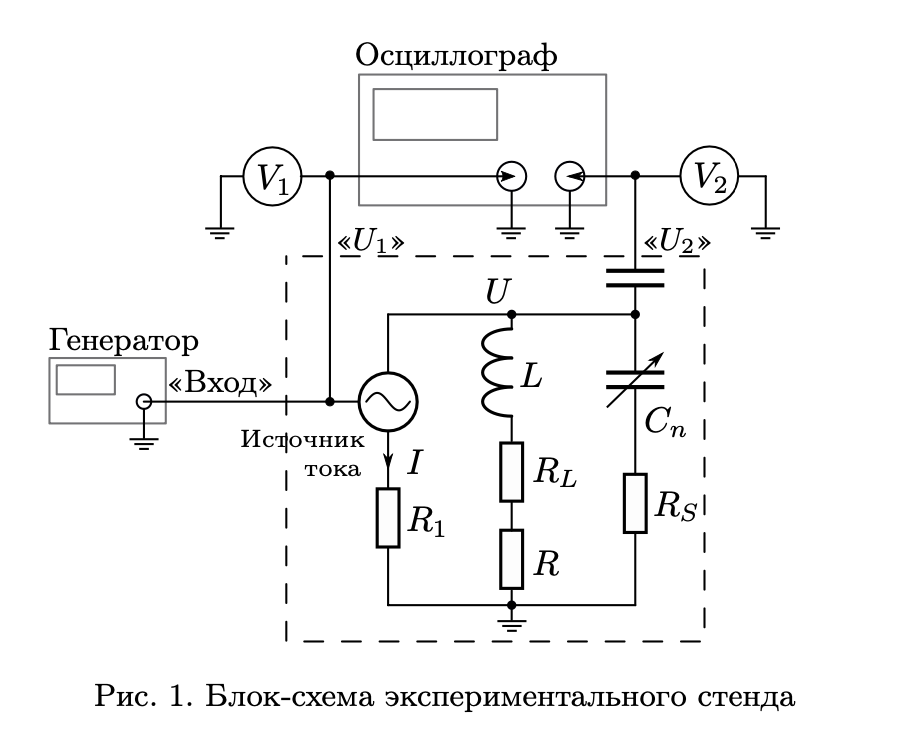
\includegraphics[width=0.8\linewidth]{im2}
\end{center}

Из данной схемы цепи ток на генераторе:

\begin{equation}
    I=\dfrac{E}{R_I}=\dfrac{E_0cos(\omega t+\varphi_0)}{R_I}=I_0cos(\omega t+\varphi_0)
\end{equation}
\begin{equation*}
    R_S=\dfrac{U_{RS}}{I}=\frac{U_{RS}}{\omega CU_{CS}}=\dfrac{1}{\omega C}tg\delta
\end{equation*}
где $R_S$ - эквивалентное последовательное сопротивление (ЭПС). Для используемых емкостей $C_n$ выполнено

\begin{equation*}
    \tg{\delta}<10^{-3} ; \; R_{\sum}=R+R_L+R_S
\end{equation*}
где $R_{\sum}$ - суммарное активное сопротивление контура.\newline
Воспользуемся методом комплексных амплитуд:

\begin{equation}
    Z_L=R_L+i\omega L; \; Z_C=R_S-i\frac{1}{\omega C}; \; Z=R_{\sum}+i\left(\omega L-d\dfrac{1}{\omega C}\right)    
\end{equation}

Тогда напряжение на контуре и токи на индуктивной и емкостной частях контура при нулевой начальной фазе можно предствить в виде:\newline
$$I_c=I\dfrac{Z_L}{Z_C+Z_L}=iQI_0\dfrac{\omega}{\omega_0}\dfrac{1-i\dfrac{R+R_L}{\rho}\dfrac{\omega_0}{\omega}}{1+iQ(\dfrac{\omega}{\omega_0}-\dfrac{\omega_0}{\omega})}$$
$$I_L=I\dfrac{Z_c}{Z_C+Z_L}=iQI_0\frac{\omega_0}{\omega}\frac{1+itg\delta}{1+iQ(\frac{\omega}{\omega_0}-\frac{\omega_0}{\omega})}$$
$$U=I\frac{Z_LZ_c}{Z_C+Z_L}=Q\rho I_0\frac{(1-i\frac{R+R_L}{\rho}\frac{\omega_0}{\omega})(1+itg\delta)}{1+iQ(\frac{\omega}{\omega_0}-\frac{\omega_0}{\omega})}$$
где $\omega_0=\frac{1}{\sqrt{LC}}$ - собственная частота, $\rho=\sqrt{\frac{L}{C}}$ - реактивное сопротивление контура, $Q=\frac{\rho} - {R_{\sum}}$ - добротность контура\newline
Рассмотрим случай, когда $|\Delta\omega|=|\omega-\omega_0|\ll\omega_0$. Тогда
\begin{equation}
    \frac{\omega}{\omega_0}-\frac{\omega_0}{\omega}=\frac{2\Delta\omega}{\omega_0}
\end{equation}
Пренебрегая поправками порядка $Q^{-2}$, получим:

\begin{equation}
    I_{C}(t) = Q\;I_{0}\frac{\omega}{\omega_{0}}\frac{\cos{(\omega t - \psi_{C}})}{\sqrt{1 + (\tau \Delta \omega)^{2}}}; \; \;  \psi_{C} = \arctg{(\tau \Delta \omega)} - \frac{\pi}{2} + \frac{R + R_{L}}{\rho}
\end{equation}

\begin{equation}
    I_{L}(t) = Q\;I_{0}\frac{\omega}{\omega_{0}}\frac{\cos{(\omega t - \psi_{L}})}{\sqrt{1 + (\tau \Delta \omega)^{2}}}; \; \;  \psi_{L} = \arctg{(\tau \Delta \omega)} + \frac{\pi}{2} - \delta
\end{equation}


\begin{equation}
    U(t) = Q\rho\;I_{0}\frac{\omega}{\omega_{0}}\frac{\cos{(\omega t - \psi_{U}})}{\sqrt{1 + (\tau \Delta \omega)^{2}}}; \; \;  \psi_{U} = \arctg{(\tau \Delta \omega)} + \frac{\omega_{0}}{\omega}\frac{R + R_{L}}{\rho} - \delta
\end{equation}
где $\tau=\frac{2L}{R_{\sum}}=\frac{2Q}{\omega_0}$ - время затухания.\newline
При резонансе, т.е. когда $\Delta\omega=0$:

$$I_C(\omega_0)=QI_0; \; \psi_C(\omega_0)=\frac{\pi}{2}-\frac{R+R_L}{\rho}$$

$$I_L(\omega_0)=QI_0; \;
\psi_L(\omega_0)=-\frac{\pi}{2}+\delta$$

$$U(\omega_0)=Q\rho I_0=Q^2R_{\sum}I_0; \;
\psi_U(\omega_0)=-\frac{R+R_L}{\rho}+\delta$$

$$\psi'_C(\omega_0)=\psi'_L(\omega_0)=\psi'_U(\omega_0)=-\tau$$

\begin{center}
    \raggedleft
        \underline{\underline{\LARGE {Выполнение}}}
\end{center}

Данные установки: $ R = 3,50  $ Ом, $ R_1 = 1008 $ Ом.

\begin{center}
    \underline{\large {\RN{1}. Измерения резонансных частот и напряжений, а также сопутствующих величин}}
\end{center}

Проведем для 7 разных конденсаторов емкости $ C_n $ измерения резонансных частот и напряжений на них, поддерживая напряжение на вольтметре 1 равным $ E = 0,2 $ В, а также вычислим дополнительные величины, следующие из наших измерений, по следующим формулам:  

\begin{equation}\label{}
L=\frac{1}{C(2\pi f)^2} \\
\end{equation}
\begin{equation}\label{}
\rho=\frac{1}{2\pi fC} \\
\end{equation}
\begin{equation}\label{}
Z_{\text{рез}}=\frac{U}{E_0}R_1
\end{equation}
\begin{equation}\label{}
Q=\frac{UR_1}{E_0}2\pi fC
\end{equation}
\begin{equation}\label{}
R_{\sum}=\frac{E_0}{UR_1}\frac{1}{(2\pi fC)^2}
\end{equation}
\begin{equation}\label{}
R_{Smax}=10^{-3}\cdot\frac{1}{\omega_0C}
\end{equation}
\begin{equation}\label{}
R_L=\frac{E_0}{UR_1}\frac{1}{(2\pi fC)^2}-R-10^{-3}\cdot\frac{1}{\omega_0C}
\end{equation}

Результаты занесём в таблицу: 
\begin{table}[h!]
\begin{tabular}{|lcccc|c|c|c|c|c|c|c|}
\hline
\multicolumn{1}{|l|}{№} & \multicolumn{1}{l|}{Сn, нФ} & \multicolumn{1}{l|}{f\_0, кГц} & \multicolumn{1}{l|}{U, В} & \multicolumn{1}{l|}{E, В} & \multicolumn{1}{l|}{L, мкГн} & \multicolumn{1}{l|}{$\rho$, Ом} & \multicolumn{1}{l|}{Zрез, Ом} & \multicolumn{1}{l|}{Q} & \multicolumn{1}{l|}{R∑, Ом} & \multicolumn{1}{l|}{Rs, Ом} & \multicolumn{1}{l|}{$R_L$, Om} \\ \hline
\multicolumn{1}{|l|}{1} & \multicolumn{1}{c|}{22,0}   & \multicolumn{1}{c|}{34,4}      & \multicolumn{1}{c|}{1,55} & 0,279                     & 972,97                       & 210,30                          & 4704,55                       & 22,37                  & 9,40                        & 0,21                        & 5,28                           \\ \hline
\multicolumn{1}{|l|}{2} & \multicolumn{1}{c|}{33,1}   & \multicolumn{1}{c|}{28,0}      & \multicolumn{1}{c|}{1,07} & 0,279                     & 976,10                       & 171,73                          & 3126,89                       & 18,21                  & 9,43                        & 0,17                        & 5,35                           \\ \hline
\multicolumn{1}{|l|}{3} & \multicolumn{1}{c|}{47,9}   & \multicolumn{1}{c|}{23,5}      & \multicolumn{1}{c|}{0,77} & 0,280                     & 957,57                       & 141,39                          & 2160,75                       & 15,28                  & 9,25                        & 0,14                        & 5,20                           \\ \hline
\multicolumn{1}{|l|}{4} & \multicolumn{1}{c|}{57,4}   & \multicolumn{1}{c|}{21,2}      & \multicolumn{1}{c|}{0,65} & 0,280                     & 981,88                       & 130,79                          & 1803,14                       & 13,79                  & 9,49                        & 0,13                        & 5,45                           \\ \hline
\multicolumn{1}{|l|}{5} & \multicolumn{1}{c|}{66,7}   & \multicolumn{1}{c|}{19,7}      & \multicolumn{1}{c|}{0,57} & 0,280                     & 978,55                       & 121,12                          & 1551,72                       & 12,81                  & 9,45                        & 0,12                        & 5,42                           \\ \hline
\multicolumn{1}{|l|}{6} & \multicolumn{1}{c|}{82,1}   & \multicolumn{1}{c|}{17,7}      & \multicolumn{1}{c|}{0,46} & 0,280                     & 984,81                       & 109,52                          & 1260,66                       & 11,51                  & 9,52                        & 0,11                        & 5,50                           \\ \hline
\multicolumn{1}{|l|}{7} & \multicolumn{1}{c|}{99,6}   & \multicolumn{1}{c|}{16,1}      & \multicolumn{1}{c|}{0,39} & 0,281                     & 981,14                       & 99,25                           & 1039,16                       & 10,47                  & 9,48                        & 0,10                        & 5,47                           \\ \hline
\multicolumn{5}{|c|}{Средние значения}                                                                                                         & 976,1                        & \multicolumn{1}{l|}{}           & \multicolumn{1}{l|}{}         & \multicolumn{1}{l|}{}  & \multicolumn{1}{l|}{}       & \multicolumn{1}{l|}{}       & 5,4                            \\ \hline
\multicolumn{5}{|c|}{Среднеквадратичная погрешность}                                                                                           & 3,4                          & \multicolumn{1}{l|}{}           & \multicolumn{1}{l|}{}         & \multicolumn{1}{l|}{}  & \multicolumn{1}{l|}{}       & \multicolumn{1}{l|}{}       & 0,04                           \\ \hline
\end{tabular}
\end{table}


\begin{center}
    \underline{\large {\RN{2}. Измерение АЧХ}}
\end{center}

Теперь измерим амплитудно-частотную характеристику для конденсаторов $ C_3, C_4 $. При этом посчитаем также измеряемые величины по отношению к резонансным $ U_0, f_0 $. Результаты сведем в таблицу:

\begin{center}

    \begin{tabular}{|l|l|l|l|lllllll}
    \cline{1-4} \cline{8-11}
    \multicolumn{1}{|c|}{$f$,кГц} & \multicolumn{1}{c|}{$U$,В} & \multicolumn{1}{c|}{$f/f_0$} & \multicolumn{1}{c|}{$U/U_0$} &  &  & \multicolumn{1}{l|}{} & \multicolumn{1}{c|}{$f$,кГц} & \multicolumn{1}{c|}{$U$,В}   & \multicolumn{1}{c|}{$f/f_0$} & \multicolumn{1}{c|}{$U/U_0$} \\ \cline{1-4} \cline{8-11} 
    19,0                        & 0,157                    & 0,805                       & 0,209                       &  &  & \multicolumn{1}{l|}{} & \multicolumn{1}{l|}{19,0}  & \multicolumn{1}{l|}{0,206} & \multicolumn{1}{l|}{0,888}  & \multicolumn{1}{l|}{0,317}  \\ \cline{1-4} \cline{8-11} 
    19,4                        & 0,159                    & 0,822                       & 0,212                       &  &  & \multicolumn{1}{l|}{} & \multicolumn{1}{l|}{19,3}  & \multicolumn{1}{l|}{0,226} & \multicolumn{1}{l|}{0,902}  & \multicolumn{1}{l|}{0,348}  \\ \cline{1-4} \cline{8-11} 
    19,8                        & 0,167                    & 0,839                       & 0,223                       &  &  & \multicolumn{1}{l|}{} & \multicolumn{1}{l|}{19,6}  & \multicolumn{1}{l|}{0,250} & \multicolumn{1}{l|}{0,916}  & \multicolumn{1}{l|}{0,385}  \\ \cline{1-4} \cline{8-11} 
    20,2                        & 0,179                    & 0,856                       & 0,239                       &  &  & \multicolumn{1}{l|}{} & \multicolumn{1}{l|}{19,8}  & \multicolumn{1}{l|}{0,277} & \multicolumn{1}{l|}{0,925}  & \multicolumn{1}{l|}{0,426}  \\ \cline{1-4} \cline{8-11} 
    20,6                        & 0,196                    & 0,873                       & 0,261                       &  &  & \multicolumn{1}{l|}{} & \multicolumn{1}{l|}{20,1}  & \multicolumn{1}{l|}{0,318} & \multicolumn{1}{l|}{0,939}  & \multicolumn{1}{l|}{0,489}  \\ \cline{1-4} \cline{8-11} 
    21,0                        & 0,215                    & 0,890                       & 0,287                       &  &  & \multicolumn{1}{l|}{} & \multicolumn{1}{l|}{20,4}  & \multicolumn{1}{l|}{0,379} & \multicolumn{1}{l|}{0,953}  & \multicolumn{1}{l|}{0,583}  \\ \cline{1-4} \cline{8-11} 
    21,4                        & 0,242                    & 0,907                       & 0,323                       &  &  & \multicolumn{1}{l|}{} & \multicolumn{1}{l|}{20,7}  & \multicolumn{1}{l|}{0,467} & \multicolumn{1}{l|}{0,967}  & \multicolumn{1}{l|}{0,718}  \\ \cline{1-4} \cline{8-11} 
    21,8                        & 0,284                    & 0,924                       & 0,379                       &  &  & \multicolumn{1}{l|}{} & \multicolumn{1}{l|}{21,1}  & \multicolumn{1}{l|}{0,619} & \multicolumn{1}{l|}{0,986}  & \multicolumn{1}{l|}{0,952}  \\ \cline{1-4} \cline{8-11} 
    22,2                        & 0,342                    & 0,941                       & 0,456                       &  &  & \multicolumn{1}{l|}{} & \multicolumn{1}{l|}{21,4}  & \multicolumn{1}{l|}{0,641} & \multicolumn{1}{l|}{1,000}  & \multicolumn{1}{l|}{0,986}  \\ \cline{1-4} \cline{8-11} 
    22,6                        & 0,426                    & 0,958                       & 0,568                       &  &  & \multicolumn{1}{l|}{} & \multicolumn{1}{l|}{21,7}  & \multicolumn{1}{l|}{0,527} & \multicolumn{1}{l|}{1,014}  & \multicolumn{1}{l|}{0,811}  \\ \cline{1-4} \cline{8-11} 
    23,0                        & 0,572                    & 0,975                       & 0,763                       &  &  & \multicolumn{1}{l|}{} & \multicolumn{1}{l|}{22,0}  & \multicolumn{1}{l|}{0,380} & \multicolumn{1}{l|}{1,028}  & \multicolumn{1}{l|}{0,585}  \\ \cline{1-4} \cline{8-11} 
    23,4                        & 0,749                    & 0,992                       & 0,999                       &  &  & \multicolumn{1}{l|}{} & \multicolumn{1}{l|}{22,3}  & \multicolumn{1}{l|}{0,298} & \multicolumn{1}{l|}{1,042}  & \multicolumn{1}{l|}{0,458}  \\ \cline{1-4} \cline{8-11} 
    23,8                        & 0,735                    & 1,008                       & 0,980                       &  &  & \multicolumn{1}{l|}{} & \multicolumn{1}{l|}{22,6}  & \multicolumn{1}{l|}{0,236} & \multicolumn{1}{l|}{1,056}  & \multicolumn{1}{l|}{0,363}  \\ \cline{1-4} \cline{8-11} 
    24,2                        & 0,549                    & 1,025                       & 0,732                       &  &  & \multicolumn{1}{l|}{} & \multicolumn{1}{l|}{22,9}  & \multicolumn{1}{l|}{0,189} & \multicolumn{1}{l|}{1,070}  & \multicolumn{1}{l|}{0,291}  \\ \cline{1-4} \cline{8-11} 
    24,6                        & 0,373                    & 1,042                       & 0,497                       &  &  &                       &                            &                            &                             &                             \\ \cline{1-4}
    25,0                        & 0,277                    & 1,059                       & 0,369                       &  &  &                       &                            &                            &                             &                             \\ \cline{1-4}
    25,4                        & 0,213                    & 1,076                       & 0,284                       &  &  &                       &                            &                            &                             &                             \\ \cline{1-4}
    25,8                        & 0,171                    & 1,093                       & 0,228                       &  &  &                       &                            &                            &                             &                             \\ \cline{1-4}
    \end{tabular}
\end{center}

\begin{center}
    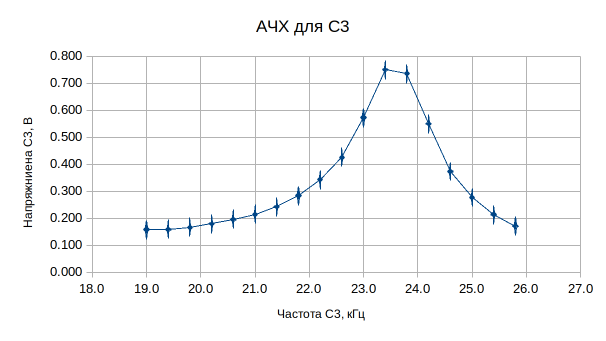
\includegraphics[width = 16 cm]{ACH_3.png}
\end{center}

\begin{center}
    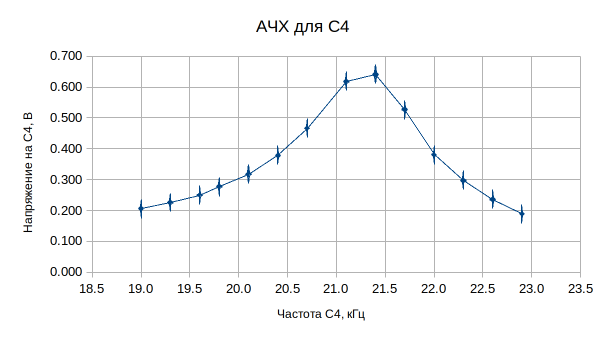
\includegraphics[width = 15 cm]{ACH_4.png}
\end{center}

\begin{center}
    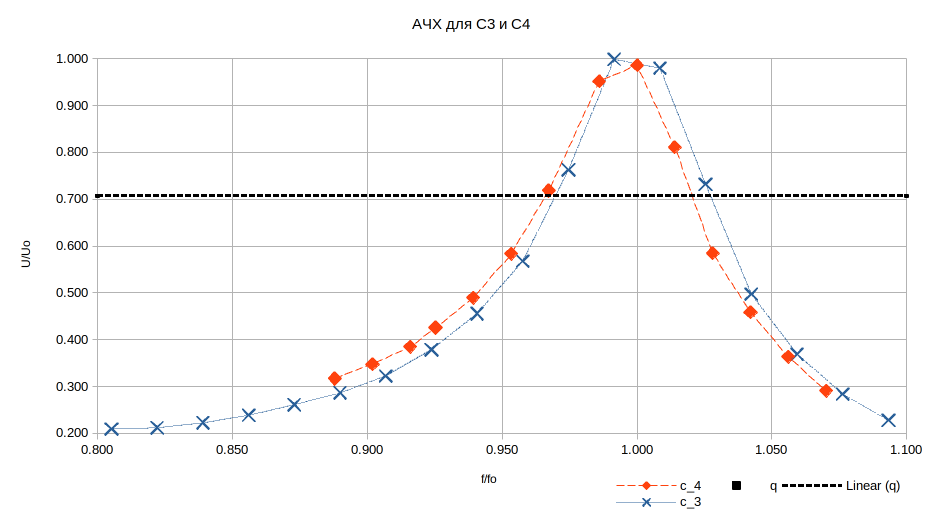
\includegraphics[width = 17 cm]{ACH_34.png}
\end{center}

Теперь найдем добротность по ширине резонансной кривой $ \delta\omega $ на 2 графике как 

\begin{equation}
    Q = \frac{\omega_{0}}{\Delta\omega}
\end{equation}  

Где $ \Delta\omega $ --- расстояние между частотами при значении напряжения $ \dfrac{1}{\sqrt{2}} \approx 0.707 $.

Получаем ответ: 

\begin{equation}
    Q_3 = (17.5 \pm \Delta Q) \qquad Q_4 = (16.7 \pm \Delta Q) \qquad \Delta Q = \frac{|Q_3 - Q_{4}|}{2} = 0.4
\end{equation}

\begin{center}
    \underline{\large {\RN{3}. Фазово-частотная характеристика}}
\end{center}

Для тех же кондесаторов определим фазово-частотную характеристику. Будем определять разность фаз между сигналами $ U(t), E(t) $ как $ \Delta\varphi = \dfrac{x}{x_0}\varphi $, где $ x, x_0 $ --- расстояния от начала отсчёта до момента обращения графиков этих значений в нуль. Результаты занесем в таблицу:

 \begin{center}
    \begin{tabular}{|l|l|l|l|l|l|llllllll}
    \cline{1-6} \cline{9-14}
    \multicolumn{1}{|c|}{$f$,кГц} & \multicolumn{1}{c|}{$f/f_0$} & $x$,cm & $x_0$,cm & $x/x_0 $ & $\varphi/\pi$ &  & \multicolumn{1}{c|}{} & \multicolumn{1}{c|}{$f$,кГц} & \multicolumn{1}{c|}{$f/f_0$} & \multicolumn{1}{l|}{$x$,cm} & \multicolumn{1}{l|}{$x_0$,cm} & \multicolumn{1}{l|}{$x/x_0 $} & \multicolumn{1}{l|}{$\varphi/\pi$} \\ \cline{1-6} \cline{9-14} 
    19,0                          & 0,81                         & 2,8    & 5,4      & 0,52     & 0,165        &  & \multicolumn{1}{l|}{} & \multicolumn{1}{l|}{19,0}    & \multicolumn{1}{l|}{0,89}    & \multicolumn{1}{l|}{2,7}    & \multicolumn{1}{l|}{5,3}      & \multicolumn{1}{l|}{0,51}     & \multicolumn{1}{l|}{0,162}        \\ \cline{1-6} \cline{9-14} 
    19,4                          & 0,82                         & 2,8    & 5,3      & 0,53     & 0,168        &  & \multicolumn{1}{l|}{} & \multicolumn{1}{l|}{19,3}    & \multicolumn{1}{l|}{0,90}    & \multicolumn{1}{l|}{2,6}    & \multicolumn{1}{l|}{5,3}      & \multicolumn{1}{l|}{0,49}     & \multicolumn{1}{l|}{0,156}        \\ \cline{1-6} \cline{9-14} 
    19,8                          & 0,84                         & 2,7    & 5,0      & 0,54     & 0,172        &  & \multicolumn{1}{l|}{} & \multicolumn{1}{l|}{19,6}    & \multicolumn{1}{l|}{0,92}    & \multicolumn{1}{l|}{2,6}    & \multicolumn{1}{l|}{5,2}      & \multicolumn{1}{l|}{0,50}     & \multicolumn{1}{l|}{0,159}        \\ \cline{1-6} \cline{9-14} 
    20,2                          & 0,86                         & 2,6    & 5,0      & 0,52     & 0,166        &  & \multicolumn{1}{l|}{} & \multicolumn{1}{l|}{19,8}    & \multicolumn{1}{l|}{0,93}    & \multicolumn{1}{l|}{2,5}    & \multicolumn{1}{l|}{5,1}      & \multicolumn{1}{l|}{0,49}     & \multicolumn{1}{l|}{0,156}        \\ \cline{1-6} \cline{9-14} 
    20,6                          & 0,87                         & 2,5    & 5,0      & 0,50     & 0,159        &  & \multicolumn{1}{l|}{} & \multicolumn{1}{l|}{20,1}    & \multicolumn{1}{l|}{0,94}    & \multicolumn{1}{l|}{2,3}    & \multicolumn{1}{l|}{5}        & \multicolumn{1}{l|}{0,46}     & \multicolumn{1}{l|}{0,146}        \\ \cline{1-6} \cline{9-14} 
    21,0                          & 0,89                         & 2,5    & 4,8      & 0,52     & 0,166        &  & \multicolumn{1}{l|}{} & \multicolumn{1}{l|}{20,4}    & \multicolumn{1}{l|}{0,95}    & \multicolumn{1}{l|}{2,1}    & \multicolumn{1}{l|}{4,9}      & \multicolumn{1}{l|}{0,43}     & \multicolumn{1}{l|}{0,136}        \\ \cline{1-6} \cline{9-14} 
    21,4                          & 0,91                         & 2,4    & 4,7      & 0,51     & 0,163        &  & \multicolumn{1}{l|}{} & \multicolumn{1}{l|}{20,7}    & \multicolumn{1}{l|}{0,97}    & \multicolumn{1}{l|}{1,8}    & \multicolumn{1}{l|}{4,8}      & \multicolumn{1}{l|}{0,38}     & \multicolumn{1}{l|}{0,119}        \\ \cline{1-6} \cline{9-14} 
    21,8                          & 0,92                         & 2,3    & 4,7      & 0,49     & 0,156        &  & \multicolumn{1}{l|}{} & \multicolumn{1}{l|}{21,1}    & \multicolumn{1}{l|}{0,99}    & \multicolumn{1}{l|}{1,1}    & \multicolumn{1}{l|}{4,7}      & \multicolumn{1}{l|}{0,23}     & \multicolumn{1}{l|}{0,074}        \\ \cline{1-6} \cline{9-14} 
    22,2                          & 0,94                         & 2,2    & 4,6      & 0,48     & 0,152        &  & \multicolumn{1}{l|}{} & \multicolumn{1}{l|}{21,4}    & \multicolumn{1}{l|}{1,00}    & \multicolumn{1}{l|}{0,4}    & \multicolumn{1}{l|}{4,6}      & \multicolumn{1}{l|}{0,09}     & \multicolumn{1}{l|}{0,028}        \\ \cline{1-6} \cline{9-14} 
    22,6                          & 0,96                         & 1,8    & 4,5      & 0,40     & 0,127        &  & \multicolumn{1}{l|}{} & \multicolumn{1}{l|}{21,7}    & \multicolumn{1}{l|}{1,01}    & \multicolumn{1}{l|}{0,6}    & \multicolumn{1}{l|}{4,6}      & \multicolumn{1}{l|}{0,13}     & \multicolumn{1}{l|}{0,042}        \\ \cline{1-6} \cline{9-14} 
    23,0                          & 0,97                         & 1,5    & 4,3      & 0,35     & 0,111        &  & \multicolumn{1}{l|}{} & \multicolumn{1}{l|}{22,0}    & \multicolumn{1}{l|}{1,03}    & \multicolumn{1}{l|}{0,8}    & \multicolumn{1}{l|}{4,5}      & \multicolumn{1}{l|}{0,18}     & \multicolumn{1}{l|}{0,057}        \\ \cline{1-6} \cline{9-14} 
    23,4                          & 0,99                         & 0,8    & 4,2      & 0,19     & 0,061        &  & \multicolumn{1}{l|}{} & \multicolumn{1}{l|}{22,3}    & \multicolumn{1}{l|}{1,04}    & \multicolumn{1}{l|}{1}      & \multicolumn{1}{l|}{4,4}      & \multicolumn{1}{l|}{0,23}     & \multicolumn{1}{l|}{0,072}        \\ \cline{1-6} \cline{9-14} 
    23,8                          & 1,01                         & 0,5    & 4,2      & 0,12     & 0,038        &  & \multicolumn{1}{l|}{} & \multicolumn{1}{l|}{22,6}    & \multicolumn{1}{l|}{1,06}    & \multicolumn{1}{l|}{1,2}    & \multicolumn{1}{l|}{4,4}      & \multicolumn{1}{l|}{0,27}     & \multicolumn{1}{l|}{0,087}        \\ \cline{1-6} \cline{9-14} 
    24,2                          & 1,03                         & 0,7    & 4,3      & 0,16     & 0,052        &  & \multicolumn{1}{l|}{} & \multicolumn{1}{l|}{22,9}    & \multicolumn{1}{l|}{1,07}    & \multicolumn{1}{l|}{1,4}    & \multicolumn{1}{l|}{4,3}      & \multicolumn{1}{l|}{0,33}     & \multicolumn{1}{l|}{0,104}        \\ \cline{1-6} \cline{9-14} 
    24,6                          & 1,04                         & 1,0    & 4,2      & 0,24     & 0,076        &  &                       &                              &                              &                             &                               &                               &                                   \\ \cline{1-6}
    25,0                          & 1,06                         & 1,2    & 4,2      & 0,29     & 0,091        &  &                       &                              &                              &                             &                               &                               &                                   \\ \cline{1-6}
    25,4                          & 1,08                         & 1,3    & 4,0      & 0,33     & 0,103        &  &                       &                              &                              &                             &                               &                               &                                   \\ \cline{1-6}
    25,8                          & 1,09                         & 1,4    & 4,0      & 0,35     & 0,111        &  &                       &                              &                              &                             &                               &                               &                                   \\ \cline{1-6}
    \end{tabular}
\end{center}

\begin{center}
    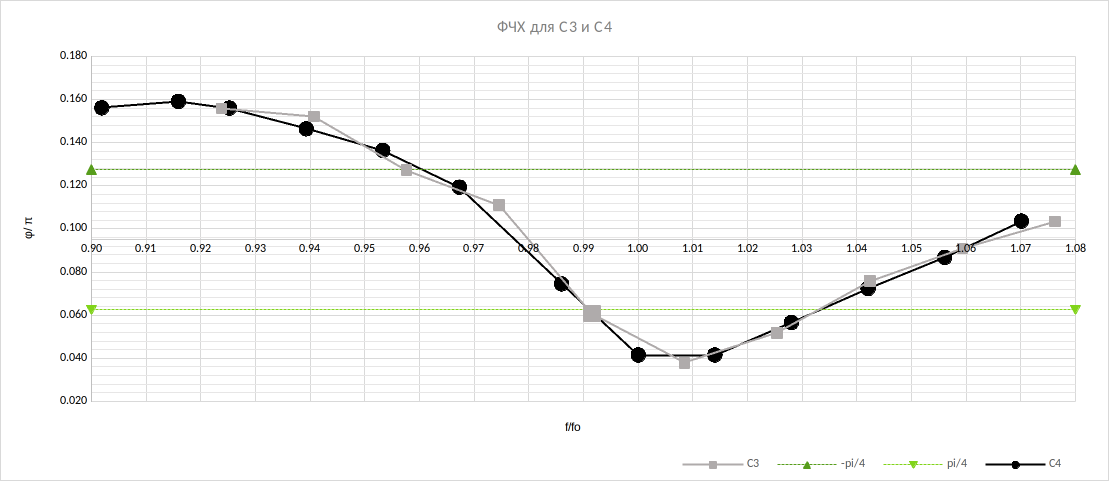
\includegraphics[width=17cm]{FCH.png}
    \caption{График фазово-частотной характеристики в осях $ \dfrac{\Delta\phi}{\pi}  \left( \dfrac{f}{f_0} \right) $}
\end{center}

Определим добротности контуров как расстояние \(\frac{1}{Q}\) между точками по оси x, в которых фаза меняется от \(\frac{-\pi}{4}\) до \(\frac{\pi}{4}\):

\begin{equation}
    Q_{3} \approx Q_{4} = 16 \pm \Delta Q \qquad \Delta Q = \frac{\sigma_{x}}{x} Q_{\text{ср}} = 0.4
\end{equation}

\newpage

\begin{center}
    \underline{\large {\RN{4}. График  зависимости $ R_L $ от $ f_{0n} $}}
\end{center}

Теперь построим график зависимости $ R_L (f_{0n}) $ и проведем прямую $ \langle R_L \rangle = 5,4 $ Ом. 

\begin{figure}[h!]
    \centering
    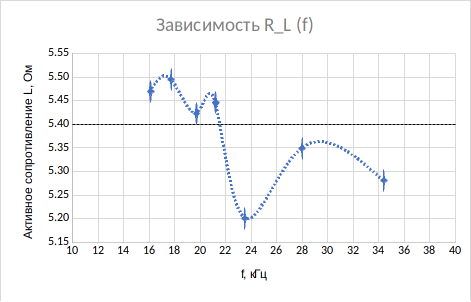
\includegraphics[width=12cm]{RL(F).png}
   \caption{График зависимости $ R_L (f_{0n}) $}
\end{figure}

\begin{center}
    \underline{\large {\RN{5}. Векторная диаграмма}}
\end{center}

Теперь построим векторную диаграмму для контура с наименьшей добротностью, т.е. для последнего --- $ Q_4= 16,9 $. 

Посчитаем ток $ I = \dfrac{E}{R_1} = \dfrac{0,2}{953} \approx 0,2 мА $. Его вектор равен сумме: $ \vec{I} = \vec{I_L} + \vec{I_C} $, причем сам $ \vec{I} $ расположен на оси абсцисс, а его компоненты расположены к нему под углами

\begin{equation}\label{}
\varphi_C = \dfrac{\pi}{2} - \dfrac{R + R_l}{\rho}, \quad \varphi_L = -\dfrac{\pi}{2} + \delta
\end{equation}

Здесь $ \delta \simeq 10^{-3}$ --- очень малый параметр установки, которым допустимо пренебречь при расчёте, однако можно изобразить для наглядности. Подсчитаем угол $ \varphi_C' =   \dfrac{R + R_L}{\rho} =\frac{3,9+5,4}{140,6}\approx 0,0665 $. 

Аналогичный угол у напряжения $ \vec{U}: \varphi_U = - \dfrac{R + R_l}{\rho} $. Т.е. оно незначительно отклоняется от оси абсцисс на отрицательный угол. Изобразим это на рисунке. 

\begin{center}
    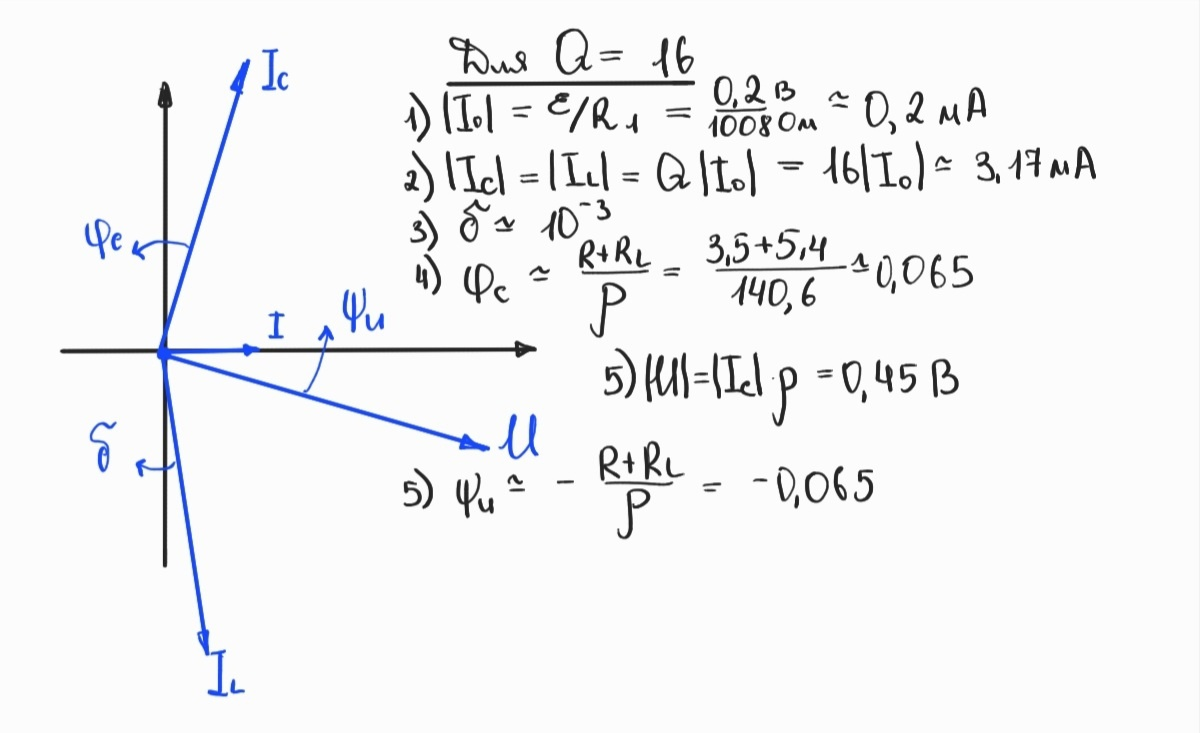
\includegraphics[width=9cm]{VDiag.jpg}
\end{center}


\begin{center}
    \raggedleft
        \underline{\underline{\LARGE {Вывод}}}
\end{center}

В данной работе мы изучили резонанс токов в параллельном контуре. С помощью непосредственных измерений, графиков АЧХ и ФЧХ мы определили добротность контуров и получили, в пределах погрешности, хорошо совпадающие результаты. 

\begin{table}[h]
    \centering
    \begin{center}
        \textbf{Таблица 6.} Значения \(Q\), полученные разными способами
    \end{center}
    \begin{tabular}{ |p{4cm}|p{4cm}|}
    \hline
        По результатам АЧХ & По результатам ФЧХ \\
    \hline
        \(Q_{3} = 17.5 \pm 0.4\) & \(Q_{3} = 16.0 \pm 0.4\) \\ \(Q_{4} = 16.7 \pm 0.4\) & \(Q_{4} = 16.0 \pm 0.4\) \\
    \hline
    \end{tabular}
\end{table} 

Проделав измерения при двух разных напряжениях $ E $, мы выяснили, что меняется только абсолютное значение резонансных амплитуд напряжения $ U $ (увеличивается при более высоком $ E $). 

В конце работы мы построили векторную диаграмму как наглядное представление "резонанса токов". 


\end{document}
